\section{Verification Approach}
%figures : 
We give a basic outline of our proof of our sufficiency theorem.

We want to show that $execute\_tree\_list (tree\_list) \in error\_states$.

We prove this by first proving the Theorem \ref{thm:etl}.

\begin{proof}[Theorem \ref{thm:etl}]
This is a proof by induction on the size of $tree\_list$.

For our base case we show that if $tree\_list$ is of length $1$, then execute\_tree\_list ($tree\_list$) $\in$ concretize\_leaf ($t$).


To prove this we use the following set property (which we verify in Coq):

\begin{theorem}
\label{thm:set2}
$\forall$ inputs $i$,
If $A \in B$ and 
$\forall x \in B$, conc\_ex($x, i$) $\in C$, then  conc\_ex($A, i$) $\in$ $C$.
\end{theorem}

If $tree\_list$ is of length $1$, we know we are executing from the initial concrete state of the system. Therefore, we consider the following properties:
\begin{itemize}
\item $init\_conc\_state \in$ 
  concretize\_root (last\_elem ($t$)). (Property $1$)
 \item $ \forall$ inputs $i$, 
 $\forall x \in$
  concretize\_root (last\_elem ($t$)),  
  conc\_ex($x, i$) $\in$ concretize\_leaf(last\_elem($t$)).
\end{itemize}

Now, using Theorem \ref{thm:set2}, we conclude that conc\_ex($init\_conc\_state$) $\in$ concretize\_leaf(last\_elem($t$)).

Our inductive hypothesis is  $execute\_tree\_list (tree\_list') \in concretize\_leaf (t')$ where $tree\_list'$ is $tree\_list$ with the last element removed and $t'$ is the last element of $tree\_list'$.

We want to show that if our inductive hypothesis holds, then $execute\_tree\_list (tree\_list) \in concretize\_leaf (t)$.

In order to prove this, we must prove the following lemma:
\begin{lemma} 
\label{lem:etl}
$execute\_tree\_list (tree\_list') \in concretize\_leaf (t)$.
\end{lemma}
\begin{proof}[Lemma \ref{lem:etl}]
We prove this using the following set property (which we verify in Coq):

\begin{theorem} \label{thm:set1}
If $A \in B$ and $B \subseteq C$, then $A \in C$.
\end{theorem}

We know:
\begin{itemize}
\item execute\_tree\_list ($t'$) $\in$
        concretize\_leaf (last\_elem($t'$)). (Inductive Hypothesis)
\item 
concretize\_leaf (last\_elem $t'$) $\subseteq$ concretize\_root (last\_elem $t$). (Property $3$)
 \end{itemize}
 
 So, using Theorem \ref{thm:set1}, we conclude that execute\_tree\_list ($t'$) $\in$ concretize\_root (last\_elem $t$). \qed
\end{proof}

Now, to prove our inductive step, we know:
\begin{itemize}
\item execute\_tree\_list (tree\_list') $\in$ concretize\_leaf ($t$). (Lemma \ref{lem:etl})
\item if $x \in$ concretize\_root($t$), then  conc\_ex($x$, get\_input (get\_pc ($l$))) $\in$ concretize\_leaf($t$),
where $l$ is a leaf of $t$. (Lemma \ref{cop})
\item concretize\_leaf($t$) $\neq \{\} $. (Property $3'$)
\end{itemize}

So, using Theorem \ref{thm:set2}, we can conclude that execute\_tree\_list ($tree\_list$) $\in$ concretize\_leaf ($t$). \qed
\end{proof}

Now, we prove our sufficiency property.

\begin{proof}[Theorem \ref{thm:sufficiency}]
We know:
\begin{itemize}
\item execute\_tree\_list ($tree\_list$) $\in$ concretize\_leaf ($t$), where $t$ is the last element of $tree\_list$. (Theorem \ref{thm:etl})
\item concretize\_leaf (last\_elem ($tree\_list$)) $\subseteq$ error\_states. (Property $2'$)
\end{itemize}
so, using Theorem \ref{thm:set1}, we conclude
execute\_tree\_list ($tree\_list$) $\in$ error\_states. \qed
\end{proof}

The reason we need Property $2'$ is because Property $2$ is not sufficient. This is because if execute\_tree\_list ($tree\_list$) $\in$ concretize\_leaf ($t$) and concretize\_leaf (last\_elem ($tree\_list$)) $\cap$ error\_states $\neq \{\}$, we could get the case where
execute\_tree\_list ($tree\_list$) $\notin$ error\_states, as shown in Figure \ref{fig:Prop2}.

\begin{figure}
\label{fig:Prop2}
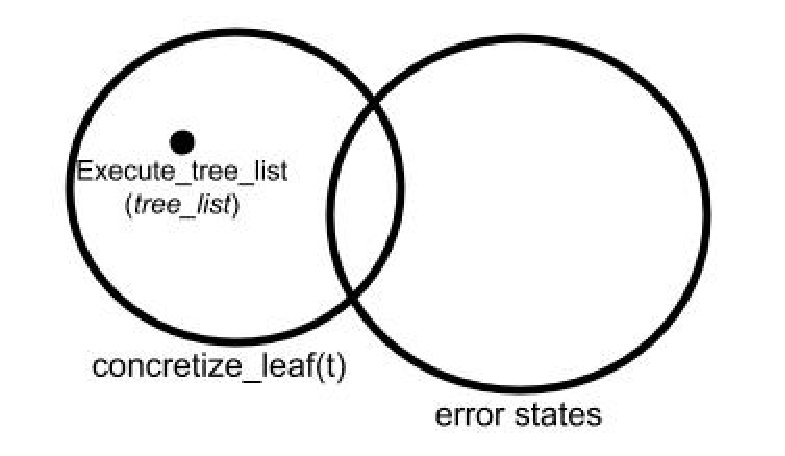
\includegraphics[width=\textwidth]{prop2.eps}
\caption{Example of Property $2$ not being sufficient to show execute\_tree\_list ($tree\_list$) $\in$ error\_states.}
\end{figure}




